\subsection{Trådløs kommunikation}\label{traadloes_komm_imp}
Den trådløse kommunikation er designet til direkte kommunikation mellem mikrokontrolleren og prototypen, hvorved exoskelettet kan styres. Herudover skal der etableres en trådløs forbindelse til en computer til debugging og test af mikrokontrolleren samt datavisualisering.   

\noindent
Til implementeringen af den trådløse kommunikation tages der ikke udgangspunkt i det oprindelige design, som er beskrevet i \autoref{sec:traadloes_komm_design}. Dette er grundet, at opsætningen af BLE kommunikationen i mikrokontrolleren er mere kompliceret end først antaget.
Af denne grund vælges det at implementere et mere simpelt og anvendeligt alternativ, bestående af to PSoC 4 M-Series Prototyping Kit boards, der ses af \autoref{fig:PSoC_4200}. Disse vil efterfølgende refereres til som gumsticks. 

\begin{figure}[H]
	\centering
	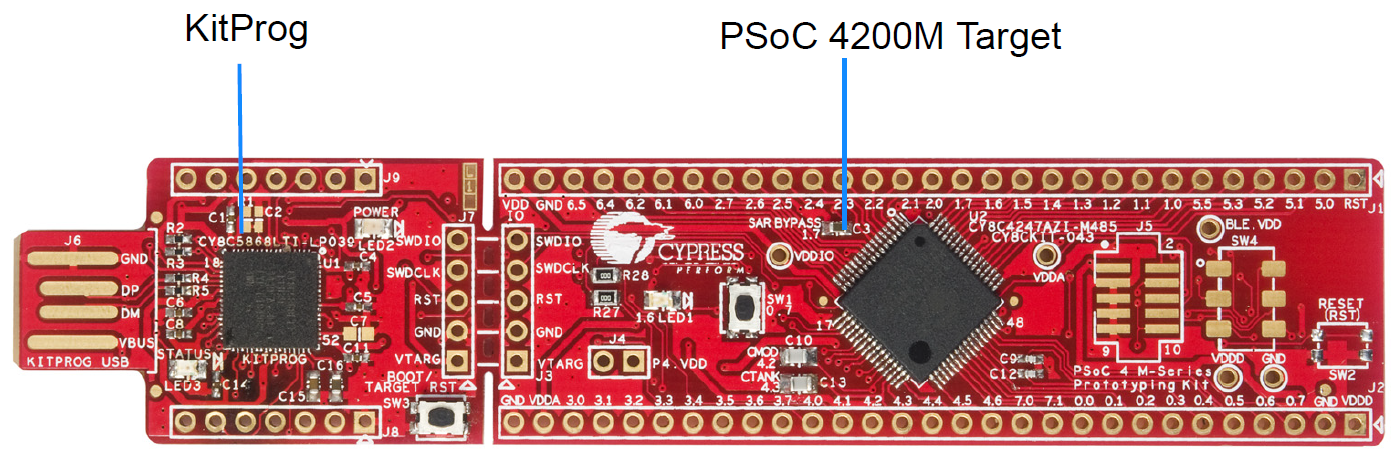
\includegraphics[width=0.8\textwidth]{figures/PSoC_4200_opdelt}
	\caption{Opbygningen af en gumstick \citep{cypresspsoc42015}.}
	\label{fig:PSoC_4200}
\end{figure}

\noindent
Gumstickens board på \autoref{fig:PSoC_4200} består af en KitProg og en PSoC 4200M enhed. KitProgen anvendes til at debugge og programmere koden. PSoC 4200M er enheden hvorpå processoren er placeret, hvor koden eksekveres. Yderligere er boardet udstyret med et EZ-BLE modul, der tillader trådløs kommunikation ved brug af BLE. 

Den ene gumstick tilkobles mikrokontrolleren via en Universal Asynchronous Receiver/Transmitter (UART)-forbindelse, der både kan sende og modtage data ved at forbinde mikrokontrollerens transmitter (TX) med gumstickens receiver (RX), og forbinde mikrokontrollerens receiver med gumstickens transmitter. 

Den anden gumstick tilsluttes computeren via en USB-forbindelse og erstatter BLE-donglen fra det oprindelige design. En illustration af, hvordan kommunikationen transmiteres i det implementerede system fremgår af \autoref{fig:Traadloes_Komm_Imp}.

\begin{figure}[H]
	\centering
	\includegraphics[width=0.8\textwidth]{figures/traadloes_komm}
	\caption{Illustration af kommunikation mellem mikrokontroller og computer. Der ses UART forbindelse til venstre, hvor der er anvendes RX og TX. Til højre ses indikeringen af tråløskommunikation ved brug af BLE \citep{cypresspsoc2015, cypresspsoc42015}.} 
	\label{fig:Traadloes_Komm_Imp}
\end{figure}

\noindent
Opsætningen, der fremgår af \autoref{fig:Traadloes_Komm_Imp} er mere anvendelig, da der findes kodeeksempler til gumsticken, hvorpå den trådløse kommunikation i forvejen er programmeret. Dertil er det ikke nødvendigt at opsætte BLE-kommunikation, men kun hvordan dataen skal videregives. 
Begge gumsticks programmeres til at 'echo' information, der modtages via BLE eller UART og transmiteres videre. Dertil vil data modtaget fra mikrokontrolleren blive videregivet til den ene gumstick, hvorpå data transmiteres trådløst til den anden gumstick. Derfra sendes data via UART til computeren. 

For at de to gumsticks kan kommunikere med hinanden, progammeres EZ-BLE modulerne til at være henholdsvis central og perifer. Dette betegner en rolle, der gives til de to gumsticks. Central er oftest en enheden med mest processorkraft og hukommelse og den perifer er oftest en enhed med mindre og ressourcebegrænset \citep{townsend2014}. I dette system er central og perifer sat op som illustreret på \autoref{fig:Traadloes_Komm_Imp}. Mikrokontrolleren bliver anset som en primær komponent, hvortil den UART-forbundne gumstick defineres som central. Gumsticken, der modtager data via BLE, bliver dermed perifer. Ved aktiv data transmission vil en indikere i form af en blå led på den centrale og perifere gumstick lyse.